%%%%%%%%%%%%%%%%%%%%%%%%%%%%%%%%%%%%%%%%%
% Diploma Project Report — Pre-Defense 1 (Sections 1–3)
% Based on the university thesis proposal template (MastersDoctoralThesis v1.6, LaTeXTemplates.com)
%%%%%%%%%%%%%%%%%%%%%%%%%%%%%%%%%%%%%%%%%

\documentclass[
11pt,
russian, % second language for the Russian and Kyrgyz abstracts
english, % main language (last option)
singlespacing,
liststotoc,
headsepline,
]{MastersDoctoralThesis}

\usepackage[nottoc]{tocbibind}
\usepackage{xcolor}
\usepackage[utf8]{inputenc}
\usepackage[T2A,T1]{fontenc} % T2A for Cyrillic (Russian and Kyrgyz), T1 for Latin

\usepackage{mathpazo} % Palatino, as in the proposal

\usepackage[round,authoryear]{natbib}
\bibliographystyle{plainnat}

\usepackage[autostyle=true]{csquotes}

\usepackage{array,tabularx,booktabs}
\usepackage{enumitem}
\setlist{itemsep=2pt,topsep=4pt,parsep=0pt}
\usepackage{tikz}
\usetikzlibrary{positioning,arrows.meta,fit}
\usepackage{listings}
\lstset{basicstyle=\ttfamily\footnotesize,breaklines=true,columns=fullflexible,frame=single,framesep=6pt}
\usepackage{textcomp}
\usepackage{float} % keep tables under their headings
\usepackage{xurl}

\newcolumntype{L}{>{\raggedright\arraybackslash}X}
\newcolumntype{P}[1]{>{\raggedright\arraybackslash}p{#1}}
\setlength{\emergencystretch}{3em}
\newenvironment{tightblock}{\small\setlength{\tabcolsep}{4pt}}{}
\newcommand{\sqm}{m\textsuperscript{2}}

\geometry{
	paper=a4paper,
	inner=2.5cm,
	outer=3.8cm,
	bindingoffset=.5cm,
	top=1.5cm,
	bottom=1.5cm,
}

\thesistitle{JK3DStudio VR: Automated Generation of Interactive Virtual Reality
Presentations from 3ds Max Interior Design Projects with a Fact-Grounded AI Guide}
\supervisor{Dr. Andrei Ermakov}
\examiner{}
\degree{Bachelor}
\author{Kiyalbek kyzy Jasmina}
\addresses{}
\keywords{virtual reality, interior design, Unreal Engine, AI guide, large language models, fact checking, Kyrgyzstan}
\university{\href{http://alatoo.edu.kg/}{Ala-Too International University}}
\department{\href{http://department.university.com}{Computer Science Department}}
\faculty{\href{http://faculty.university.com}{Foundations of Creativity Industries}}

\AtBeginDocument{
\hypersetup{pdftitle=\ttitle}
\hypersetup{pdfauthor=\authorname}
\hypersetup{pdfkeywords=\keywordnames}
}

\begin{document}

\frontmatter
\pagestyle{plain}

%----------------------------------------------------------------------------------------
%	TITLE PAGE
%----------------------------------------------------------------------------------------

\begin{titlepage}
\begin{center}

\vspace*{.06\textheight}
{\scshape\LARGE \univname\par}\vspace{1.5cm}

\HRule \\[0.4cm]
{\huge \bfseries \ttitle\par}\vspace{0.4cm}
\HRule \\[1.5cm]

\begin{minipage}[t]{0.4\textwidth}
\begin{flushleft} \large
\emph{Author:}\\
\authorname
\end{flushleft}
\end{minipage}
\begin{minipage}[t]{0.4\textwidth}
\begin{flushright} \large
\emph{Supervisor:} \\
\supname
\end{flushright}
\end{minipage}\\[3cm]

\vfill

\large \textit{A diploma project report for the degree of \degreename}\\[0.3cm]
\textit{First pre-defense: Sections 1--3}\\[0.4cm]
\deptname\\[2cm]

\vfill

{\large December 2026}\\[4cm]

\vfill
\end{center}
\end{titlepage}

%----------------------------------------------------------------------------------------
%	DECLARATION PAGE
%----------------------------------------------------------------------------------------

\begin{declaration}
\addchaptertocentry{\authorshipname}
\noindent I, \authorname, declare that this report titled, \enquote{\ttitle} and the work presented in it are my own. I confirm that:

\begin{itemize}
\item This work was done wholly or mainly while in candidature for a degree at this university.
\item Where I have consulted the published work of others, this is always clearly attributed.
\item Where I have quoted from the work of others, the source is always given. With the exception of such quotations, this report is entirely my own work.
\item I have acknowledged all main sources of help, including the AI tools listed in Appendix~\ref{AppendixA}.
\item Where the work is based on work done by myself jointly with others, I have made clear exactly what was done by others and what I have contributed myself.\\
\end{itemize}

\noindent Signed:\\
\rule[0.5em]{25em}{0.5pt}

\noindent Date:\\
\rule[0.5em]{25em}{0.5pt}
\end{declaration}

\cleardoublepage

%----------------------------------------------------------------------------------------
%	ABSTRACTS (ENGLISH, RUSSIAN, KYRGYZ)
%----------------------------------------------------------------------------------------

\begin{abstract}
\addchaptertocentry{\abstractname}
Interior design clients in Kyrgyzstan usually approve a project from 360\textdegree{} panoramas and renders. The designer chooses the camera, and wide-angle lenses and idealised lighting make rooms look larger and brighter than they will be. As a result, clients misjudge room size, light and how doors and furniture actually open, and these mistakes surface only during renovation.

This report presents \textit{JK3DStudio VR}, a tool that turns a finished 3ds Max interior project into an interactive virtual reality (VR) presentation. The client walks through the future apartment at 1:1 scale, opens doors by hand, switches light per room, changes the time of day and colour temperature, and is guided by an AI guide in Russian and English. The guide speaks only facts taken from a project passport that the designer approves.

The system has three parts: an Unreal Engine 5.8 editor plugin that prepares the scene semi-automatically from a naming standard, a VR application for PICO 4 Ultra, and an AI Gateway backend (FastAPI, PostgreSQL) for speech generation, fact checking and text-to-speech. Similar interactive tours abroad are produced manually and cost from USD 10{,}000; no comparable service for design projects was found in Kyrgyzstan. The novelty is fast preparation, honest scale and light, and a fact-grounded AI guide adapted to the local market. A working prototype of the VR application and a tested backend are presented at the first pre-defense.

\medskip\noindent\textbf{Keywords:} virtual reality, interior design, Unreal Engine, AI guide, large language models, Kyrgyzstan.

\end{abstract}

\begin{extraAbstract}
\addchaptertocentry{Abstract in Russian}
\begin{otherlanguage}{russian}
В Кыргызстане клиент дизайн-студии обычно утверждает проект по 360\textdegree-панорамам и рендерам. Ракурс выбирает дизайнер, а широкоугольная камера и <<идеальный>> свет делают комнаты визуально больше и светлее, чем в реальности. В результате клиент неверно оценивает размеры, освещение и то, как открываются двери и мебель, а ошибки обнаруживаются только во время ремонта.

В работе представлен JK3DStudio VR "--- инструмент, который превращает готовый дизайн-проект из 3ds Max в интерактивную VR-презентацию. Клиент ходит по будущей квартире в масштабе 1:1, открывает двери рукой, включает свет по комнатам, меняет время суток и цветовую температуру. ИИ-гид на русском и английском рассказывает о проекте и говорит только факты из паспорта проекта, утверждённого дизайнером.

Система состоит из трёх частей: плагина для редактора Unreal Engine 5.8, который полуавтоматически готовит сцену по стандарту имён, VR-приложения для очков PICO 4 Ultra и серверной части AI Gateway (FastAPI, PostgreSQL) для генерации речи, проверки фактов и озвучки. За рубежом подобные интерактивные туры делают вручную, их стоимость "--- от 10\,000 долларов США; аналогичной услуги для дизайн-проектов в Кыргызстане не найдено. Новизна "--- быстрая подготовка, честные масштаб и свет и ИИ-гид, опирающийся на факты, с адаптацией к местному рынку. На первой предзащите демонстрируются рабочий прототип VR-приложения и протестированная серверная часть.

\medskip\noindent\textbf{Ключевые слова:} виртуальная реальность, дизайн интерьера, Unreal Engine, ИИ-гид, большие языковые модели, Кыргызстан.

\end{otherlanguage}
\end{extraAbstract}

\begin{extraAbstract}
\addchaptertocentry{Abstract in Kyrgyz}
\begin{otherlanguage}{russian}
Кыргызстанда дизайн-студиянын кардарлары долбоорду көбүнчө 360\textdegree{} панорамалар жана рендерлер аркылуу бекитет. Камеранын бурчун дизайнер тандайт, ал эми кең бурчтуу камера жана <<идеалдуу>> жарык бөлмөлөрдү чындыгындагыдан чоңураак жана жарыгыраак кылып көрсөтөт. Натыйжада кардар бөлмөнүн өлчөмүн, жарыкты, эшик менен эмеректердин кантип ачыларын туура эмес баалайт, ал эми мындай каталар оңдоо иштеринин учурунда гана билинет.

Бул иште JK3DStudio VR сунушталат "--- 3ds Max программасында даярдалган дизайн-долбоорду интерактивдүү виртуалдык чындык (VR) презентациясына айландыруучу курал. Кардар келечектеги батирди 1:1 масштабда кыдырып, эшиктерди колу менен ачат, ар бир бөлмөдө жарыкты күйгүзөт, күндүн убактысын жана жарыктын түс температурасын өзгөртөт. Орус жана англис тилдеринде сүйлөгөн ЖИ-гид дизайнер бекиткен долбоордун паспортундагы фактыларды гана айтат.

Система үч бөлүктөн турат: аталыштардын стандарты боюнча сахнаны жарым-автоматтык түрдө даярдаган Unreal Engine 5.8 плагини, PICO 4 Ultra көз айнегине арналган VR-тиркеме жана сүйлөө текстин түзүү, фактыларды текшерүү жана үн берүү үчүн AI Gateway сервердик бөлүгү (FastAPI, PostgreSQL). Чет өлкөлөрдө мындай интерактивдүү турлар кол менен жасалат жана баасы 10\,000 АКШ долларынан башталат. Кыргызстанда дизайн-долбоорлор үчүн мындай кызмат табылган жок. Жаңылыгы "--- тез даярдоо, чыныгы масштаб жана жарык, ошондой эле жергиликтүү рынокко ыңгайлаштырылган, фактыларга таянган ЖИ-гид. Биринчи алдын ала коргоодо VR-тиркеменин иштеген прототиби жана текшерилген сервердик бөлүгү көрсөтүлөт.

\medskip\noindent\textbf{Негизги сөздөр:} виртуалдык чындык, интерьер дизайны, Unreal Engine, ЖИ-гид, чоң тил моделдери, Кыргызстан.

\end{otherlanguage}
\end{extraAbstract}

%----------------------------------------------------------------------------------------
%	LISTS
%----------------------------------------------------------------------------------------

\tableofcontents
\listoffigures
\listoftables

\begin{abbreviations}{ll}
\textbf{AI} & \textbf{A}rtificial \textbf{I}ntelligence\\
\textbf{API} & \textbf{A}pplication \textbf{P}rogramming \textbf{I}nterface\\
\textbf{DSR} & \textbf{D}esign \textbf{S}cience \textbf{R}esearch\\
\textbf{FPS} & \textbf{F}rames \textbf{P}er \textbf{S}econd\\
\textbf{FR} & \textbf{F}unctional \textbf{R}equirement\\
\textbf{HMD} & \textbf{H}ead-\textbf{M}ounted \textbf{D}isplay\\
\textbf{LLM} & \textbf{L}arge \textbf{L}anguage \textbf{M}odel\\
\textbf{MCP} & \textbf{M}odel \textbf{C}ontext \textbf{P}rotocol\\
\textbf{MVP} & \textbf{M}inimum \textbf{V}iable \textbf{P}roduct\\
\textbf{NFR} & \textbf{N}on-\textbf{F}unctional \textbf{R}equirement\\
\textbf{RAG} & \textbf{R}etrieval-\textbf{A}ugmented \textbf{G}eneration\\
\textbf{RQ} & \textbf{R}esearch \textbf{Q}uestion\\
\textbf{SUS} & \textbf{S}ystem \textbf{U}sability \textbf{S}cale\\
\textbf{TTS} & \textbf{T}ext-\textbf{T}o-\textbf{S}peech\\
\textbf{UE} & \textbf{U}nreal \textbf{E}ngine\\
\textbf{VR} & \textbf{V}irtual \textbf{R}eality\\
\end{abbreviations}

%----------------------------------------------------------------------------------------
%	SECTIONS 1–3
%----------------------------------------------------------------------------------------

\mainmatter
\pagestyle{thesis}

\chapter{Problems} % Section 1
\label{Chapter1}

Clients approve interior design projects from images that hide true scale, true light and how the space works in use. The cost of a wrong decision appears later, during renovation.

%----------------------------------------------------------------------------------------
\section{Problem Statement}

In Kyrgyzstan most interior design studios deliver a project as renders and 360\textdegree{} panoramas made in 3ds Max with Corona Renderer and shared by link. This observation comes from the author's own practice; it will be confirmed by interviews with 5--10 Bishkek studios (Section~\ref{sec:scope}). The format creates four problems:

\begin{enumerate}
\item \textbf{Distorted scale.} The designer chooses the camera position and focal length. A wide-angle lens and a camera placed in a corner or behind a wall make a room look larger, and narrow passages and conflicts stay out of frame.
\item \textbf{Idealised light.} Sun and artificial light are set for beauty, not for the real orientation, season and time of day. The client cannot see the room at 19:00 in December, or the difference between 2700\,K and 6500\,K lamps.
\item \textbf{Untested movement.} Doors and fronts are usually shown open or hidden. Whether a door hits a cabinet, or a drawer hits an oven handle, is found only on site.
\item \textbf{Weak understanding.} Drawings and separate images do not add up to one space in the client's mind. The designer repeats the same explanations, and the client still signs the project without fully understanding it.
\end{enumerate}

A related survey in real estate shows the scale of the issue: 33\% of buyers said a property did not match their expectations, with size as the main reason, and 71\% were disappointed at a viewing \citep{movestreets2021}.

%----------------------------------------------------------------------------------------
\section{Market Research}

\paragraph{Global.} The virtual tour market is forecast to reach USD 7.35 billion by 2031, growing 29.8\% a year; the real estate segment grows 29.2\% a year and Asia-Pacific is the fastest region at 30.5\% \citep{kbv2025}. Hand-built interactive Unreal Engine tours from studios such as ArchiCGI start at about USD 10{,}000 \citep{archicgi}.

\paragraph{Kyrgyzstan.} In the first half of 2026, 837.8 thousand \sqm{} of housing was commissioned (+7.5\%) \citep{econkg2026}, while sales slowed: 2{,}686 apartments were sold in Bishkek in the first quarter of 2026 and the policy rate rose to 12\% \citep{kaktus2026}. More supply and slower sales mean stronger competition for each buyer. Part of the buyers, from Russia and Kazakhstan, buy remotely and need an honest view in advance. Table~\ref{tab:kg-offers} lists what is offered locally.

\begin{table}[H]
\centering
\begin{tightblock}
\begin{tabularx}{\textwidth}{P{3.6cm} P{3.6cm} L}
\toprule
\textbf{Offer in Kyrgyzstan} & \textbf{Example} & \textbf{Limitation} \\
\midrule
360\textdegree{} panoramas and renders from 3ds Max / Corona & Most design studios (author's observation) & Designer picks the view; no 1:1 scale; no interaction \\
3D visualisation inside a design project & NeoStyle, USD 10--35 per \sqm{} & Images only \\
Matterport scanning & Pro3D, about 5{,}000 KGS for up to 100 \sqm{} & Works only for spaces that already exist, not for a project before renovation \\
\enquote{3D tours and VR} for interiors & Liberty.kg & Format not described publicly \\
\bottomrule
\end{tabularx}
\end{tightblock}
\caption{Visualisation services for interiors in Kyrgyzstan}
\label{tab:kg-offers}
\end{table}

In open sources no interactive VR service with an AI guide for design projects was found in Kyrgyzstan. This is a limitation of desk research and is checked by interviews.

%----------------------------------------------------------------------------------------
\section{Literature Review}

\paragraph{VR improves non-experts' understanding of a design.} \citet{serpa2020} ran two experiments with architects and real clients, presenting the same project traditionally and in head-mounted VR; clients understood the project more accurately in VR. \citet{alawwad2024} interviewed eight clients and four designers of an interior agency in Medina and found VR useful for presenting interior outputs, more so for commercial than for residential projects. \citet{kurpinar2025} studied immersive VR inside a working architectural office and its effect on presentations to clients.

\paragraph{Adoption barriers remain.} A study of real design reviews found that architects and client representatives still resist VR even though it supports shared understanding \citep{chalmersvr}. Reported barriers include preparation effort, equipment and disruption of the usual workflow. This supports the focus of this work on \emph{preparation time}, not only on visual quality.

\paragraph{Scale perception in VR is good but not perfect.} A review of 33 studies found that egocentric distances in VR were estimated at about 73--74\% of the modelled distance on average \citep{renner2013}. Newer headsets reduce the gap but do not remove it \citep{kelly2022,creemregehr2023}. For this project it means that 1:1 scale and correct eye height are necessary, and that scale perception must be evaluated rather than assumed.

\paragraph{From design models to game engines.} Several papers describe workflows from BIM to VR through game engines: Revit with Twinmotion and Datasmith \citep{wijerathna2024}, heritage BIM to Unity \citep{pybus2019}, and an IFC-based interactive tool with two-way data exchange \citep{nandavar2018}. These workflows are manual or semi-automatic, start from BIM (Revit, IFC) rather than 3ds Max, and do not add opening mechanics, per-room light scenarios or a guide.

\paragraph{AI guides and hallucination.} Large language models can produce fluent but factually wrong text \citep{huang2023}. Retrieval-augmented generation grounds the output in external sources but still fails when retrieval or generation fails \citep{huang2023,alansari2025}. Checking the generated text against a trusted source after generation is one of the main mitigation methods. For a guide that talks to a buyer, an invented area or ceiling height is a real harm, which motivates the \enquote{approved passport and Fact Guard} design described in Chapter~\ref{Chapter3}.

%----------------------------------------------------------------------------------------
\section{Review of Existing Solutions}

Table~\ref{tab:analogues} compares the main tools and services on the functions this project targets.

\begin{table}[H]
\centering
\begin{tightblock}
\footnotesize
\begin{tabularx}{\textwidth}{P{2.7cm} P{2.3cm} P{1.6cm} P{1.1cm} P{1.1cm} L}
\toprule
\textbf{Solution} & \textbf{Type} & \textbf{Preparation} & \textbf{Doors by hand} & \textbf{Light per room} & \textbf{AI guide; price} \\
\midrule
Twinmotion (Epic) & Visualiser + VR & Fast & No & No & No; subscription \\
Enscape (Chaos) & Revit/SketchUp plugin & Fast, no 3ds Max & No & No & No; USD 575--1{,}139/yr \\
Chaos Vantage & Real-time V-Ray/Corona viewer & Fast & No & Light editing & No; about USD 995/yr \\
Lumion & Visualiser & Medium & No & No & No; about USD 19--96/mo \\
Autodesk Workshop XR & Shared BIM review & Fast & No & No & No; USD 1{,}075/yr \\
ArchiCGI, Maverickframe & Manual Unreal work & Weeks & On order & On order & No; from USD 10{,}000 \\
PropVR & Digital twins & Weeks & On order & On order & Sales avatar; on request \\
Matterport & Scan of existing spaces & Fast & No & No & No; subscription \\
\midrule
\textbf{JK3DStudio VR} & \textbf{Unreal plugin for 3ds Max studios} & \textbf{Target $\le$ 30 min} & \textbf{Yes} & \textbf{Yes} & \textbf{Yes, fact-checked, RU/EN; affordable} \\
\bottomrule
\end{tabularx}
\end{tightblock}
\caption{Existing solutions compared with JK3DStudio VR}
\label{tab:analogues}
\end{table}

%----------------------------------------------------------------------------------------
\section{Research Gap}

Fast tools (Twinmotion, Enscape, Vantage) give real-time VR but no interaction with doors, furniture and room light, and no guide. Interactive tours exist only as manual studio work costing weeks and from USD 10{,}000. None of the reviewed tools starts from a 3ds Max and Corona project, which is the common local workflow. This work addresses that gap: \textbf{interactive, honest VR from a 3ds Max project, prepared in minutes, with a guide that cannot invent facts, for the Kyrgyz market.}
 % Section 1. Problems
\chapter{Aim and Objectives} % Section 2
\label{Chapter2}

The aim is to cut the time to turn a 3ds Max interior project into an honest, interactive VR presentation from days to under 30 minutes, with an AI guide that states only approved facts.

%----------------------------------------------------------------------------------------
\section{Aim}

To design, implement and evaluate JK3DStudio VR: a system that semi-automatically converts a 3ds Max interior design project into an interactive 1:1 VR presentation with physically operable doors, per-room lighting and time of day, and a bilingual (Russian and English) AI guide grounded in a designer-approved project passport.

%----------------------------------------------------------------------------------------
\section{Objectives}

\begin{enumerate}[label=\textbf{O\arabic*.}]
\item \textbf{Preparation pipeline.} Build an Unreal Engine 5.8 editor plugin that imports a Datasmith scene and sets collision, walkable zones, movable elements and light groups from a naming standard, with manual correction. Target: a new project ready in $\le$ 30 minutes.
\item \textbf{Interactive VR application.} Implement 1:1 walking (stick, snap turn, room-scale) with wall and furniture collision, doors opened with either hand from both sides, per-room light on/off and colour temperature 2700--6500\,K, and a sun position slider from 06:00 to 22:00. Target: $\ge$ 72 FPS on PICO 4 Ultra via PICO Connect.
\item \textbf{Fact-grounded AI guide.} Build an AI Gateway service that turns the designer's key points and the approved passport into guide speech in Russian and English, checks every number against the passport (Fact Guard) and produces voice audio. Target: no unsupported numbers in approved scripts.
\item \textbf{Evaluation.} Evaluate preparation time, performance, factual accuracy and user perception with designers and clients. Target: tests on at least 2 projects and 5 users.
\end{enumerate}

%----------------------------------------------------------------------------------------
\section{Research Questions}

\begin{description}[leftmargin=1.2cm,style=nextline]
\item[RQ1] Can a naming standard plus geometric rules prepare a 3ds Max interior for interactive VR in $\le$ 30 minutes, with $\ge$ 95\% of movable elements detected when the standard is followed?
\item[RQ2] Does a fact-checking layer over an LLM remove unsupported numerical claims from the guide's speech compared with generation without checking?
\item[RQ3] Do clients judge room size, light and door conflicts more accurately in the interactive VR presentation than from renders and 360\textdegree{} panoramas of the same project?
\end{description}

RQ1 and RQ2 are answered by measurement and automated tests. RQ3 is answered by a user study before the final defense.

%----------------------------------------------------------------------------------------
\section{Scope and Constraints}
\label{sec:scope}

\begin{itemize}
\item \textbf{In scope:} apartments and small spaces modelled in 3ds Max 2024 with Corona 11; PC-tethered VR (PICO 4 Ultra via PICO Connect and SteamVR); Russian and English.
\item \textbf{Out of scope for the diploma:} Archicad and Revit import, Blender, a standalone headset build, live voice questions, Kyrgyz voice, window view generated from the address.
\item \textbf{Constraints:} one developer; a consumer laptop with an NVIDIA GPU; the Unreal Engine licence is free under USD 1 million revenue; the demonstration must run offline.
\end{itemize}

%----------------------------------------------------------------------------------------
\section{Stakeholders}

\begin{table}[H]
\centering
\begin{tightblock}
\begin{tabularx}{\textwidth}{P{4.2cm} P{3.6cm} L}
\toprule
\textbf{Stakeholder} & \textbf{Role} & \textbf{Main need} \\
\midrule
Interior designer or small studio & Prepares and runs the presentation & Fast preparation; control over what the guide says \\
Client and family & Walk through the project & Honest scale and light; easy controls \\
Developer or real estate agency & Secondary buyer & Remote viewing for buyers from abroad \\
System administrator (author) & Runs the AI Gateway & Secure keys, logs, backups \\
External services & LLM and TTS providers & API access within budget \\
\bottomrule
\end{tabularx}
\end{tightblock}
\caption{Stakeholders and their needs}
\label{tab:stakeholders}
\end{table}

%----------------------------------------------------------------------------------------
\section{Functional Requirements}

Priority: M = must for the MVP, S = should, C = could (after the diploma).

{\begin{tightblock}\footnotesize
\begin{longtable}{P{1.1cm} P{6.3cm} P{0.9cm} P{4.6cm}}
\caption{Functional requirements}\label{tab:fr}\\
\toprule
\textbf{ID} & \textbf{Requirement} & \textbf{Prio.} & \textbf{Acceptance criterion} \\
\midrule
\endfirsthead
\toprule
\textbf{ID} & \textbf{Requirement} & \textbf{Prio.} & \textbf{Acceptance criterion} \\
\midrule
\endhead
FR-01 & Import a Datasmith scene and set collision on all meshes & M & All meshes have collision; walls block the player \\
FR-02 & Build walkable zones on floors only; designer can add or remove a zone & M & No zone on roof or furniture; door openings walkable \\
FR-03 & Detect doors, windows and fronts by the naming standard & M & $\ge$ 95\% found on a scene that follows the standard \\
FR-04 & Open a door with either controller from both sides; a door pushes the player back & M & Tested on all doors of the pilot apartment \\
FR-05 & Five opening techniques (swing, slide, fold, lift, drop) with parts and limits & S & Each technique works on one test object \\
FR-06 & Check openings for collisions and report conflicts & S & Finds 100\% of planted conflicts in a test scene \\
FR-07 & Group lights by room from \texttt{ROOM\_<room>\_FLOOR} and object names & M & Every light assigned to a room or reported \\
FR-08 & Per-room light on/off, all on/off, colour temperature 2700--6500\,K remembered per room & M & Value restored after leaving and returning to a room \\
FR-09 & Sun position by time of day, 06:00--22:00 & M & Shadow direction changes with the slider \\
FR-10 & Light scenarios per room (main, secondary, decorative) & S & Switch cycles 1, 2, 3, all on, all off \\
FR-11 & Project passport auto-filled; designer edits and approves; required fields block the show & M & Show cannot start with an empty required field \\
FR-12 & Generate guide speech in Russian and English from key points and passport & M & Script exists for each room in both languages \\
FR-13 & Fact Guard: every number in the speech exists in the passport & M & Unsupported numbers are rejected \\
FR-14 & Text-to-speech audio and subtitles in VR & M & Audio plays with a matching subtitle \\
FR-15 & Guide character follows the client, stays in view and does not block objects & M & Stays left of the view; still while the menu is open \\
FR-16 & Designer screen with plan, client position and controls; mirror to TV & S & Designer moves the client to another room \\
FR-17 & Finish variants A/B switched in VR & S & Floor variant changes in under 1 s \\
FR-18 & Post-show report (route, time per room, actions) as PDF & C & PDF generated after a session \\
\bottomrule
\end{longtable}
\end{tightblock}}

%----------------------------------------------------------------------------------------
\section{Non-Functional Requirements}

\begin{table}[H]
\centering
\begin{tightblock}
\begin{tabularx}{\textwidth}{P{1.4cm} P{3.0cm} L}
\toprule
\textbf{ID} & \textbf{Quality} & \textbf{Measurable target} \\
\midrule
NFR-01 & Performance & $\ge$ 72 FPS in VR, goal 90, measured with \texttt{stat fps} on the pilot apartment \\
NFR-02 & Preparation time & New project ready for VR in $\le$ 30 minutes \\
NFR-03 & Responsiveness & Light, temperature or time change visible in $\le$ 1 s \\
NFR-04 & Accuracy & No unsupported numbers in approved guide scripts \\
NFR-05 & Availability of demo & Full show runs with no internet connection \\
NFR-06 & Security & API keys only on the server; HTTPS in production; no keys in the repository \\
NFR-07 & Privacy & Client name and address stored only with consent; session data deleted on request \\
NFR-08 & Usability & SUS score $\ge$ 68 from test users \\
NFR-09 & Comfort & No user stops a 10-minute session because of motion sickness \\
NFR-10 & Maintainability & Adding a language takes 3 steps (code, translation, voice) and no code change \\
NFR-11 & Reproducibility & Backend runs with one \texttt{docker compose up} following the README \\
\bottomrule
\end{tabularx}
\end{tightblock}
\caption{Non-functional requirements}
\label{tab:nfr}
\end{table}

%----------------------------------------------------------------------------------------
\section{Traceability}

\begin{table}[H]
\centering
\begin{tightblock}
\footnotesize
\begin{tabularx}{\textwidth}{P{0.9cm} P{4.0cm} P{3.4cm} L}
\toprule
\textbf{Obj.} & \textbf{Requirements} & \textbf{Component} & \textbf{Test or evidence} \\
\midrule
O1 & FR-01--FR-03, FR-05--FR-07, FR-11, NFR-02 & Editor plugin (Python, Editor Utility) & Timed preparation of 2 projects; detection rate \\
O2 & FR-04, FR-08--FR-10, FR-15--FR-17, NFR-01, NFR-03, NFR-09 & VR application (Blueprint) & FPS log; in-headset checklist; comfort questionnaire \\
O3 & FR-12--FR-14, NFR-04--NFR-07, NFR-10, NFR-11 & AI Gateway (FastAPI, PostgreSQL) & Automated tests: Fact Guard negative cases, API tests \\
O4 & NFR-08, RQ1--RQ3 & Whole system & User study, SUS, interviews \\
\bottomrule
\end{tabularx}
\end{tightblock}
\caption{Traceability from objectives to requirements, components and tests}
\label{tab:trace}
\end{table}
 % Section 2. Aim and Objectives
\chapter{Methods and Material} % Section 3
\label{Chapter3}

The system is built as three parts: an Unreal Engine editor plugin, a VR application and an AI Gateway backend. At the first pre-defense the VR application is a working prototype, the plugin is partly automated by Python scripts, and the backend is implemented and covered by automated tests.

%----------------------------------------------------------------------------------------
\section{Methodology}

The work follows Design Science Research: build an artefact that solves a stated problem, then evaluate it against measurable criteria. Development is iterative, in weekly cycles, and each cycle ends with an in-headset test on PICO 4 Ultra. Every issue is logged as problem, cause, fix and result; more than 50 such entries were recorded between 11 and 19 November 2026. Features were first built by hand on one pilot apartment and then automated. Table~\ref{tab:eval} links each research question to its method.

\begin{table}[H]
\centering
\begin{tightblock}
\begin{tabularx}{\textwidth}{P{1.0cm} L P{4.2cm}}
\toprule
\textbf{RQ} & \textbf{Method} & \textbf{Data} \\
\midrule
RQ1 & Timed preparation of 2 projects; count of detected versus actual movable elements & Stopwatch log, detection report \\
RQ2 & Generate guide scripts with and without Fact Guard; count unsupported numbers & Automated test results \\
RQ3 & Within-subject study: the same project shown as renders/360\textdegree{} and in VR; participants estimate room size, find planted door conflicts and rate light & Questionnaire, error in size estimates, SUS, comfort rating \\
\bottomrule
\end{tabularx}
\end{tightblock}
\caption{Evaluation methods by research question}
\label{tab:eval}
\end{table}

%----------------------------------------------------------------------------------------
\section{System Architecture}

The source of truth is the 3ds Max scene with a naming standard. Datasmith carries geometry, materials and lights into Unreal Engine. The editor plugin prepares the level and writes the project passport. The VR application runs the show, and the AI Gateway turns the approved passport and the designer's key points into checked speech and audio (Figure~\ref{fig:arch}).

\begin{figure}[H]
\centering
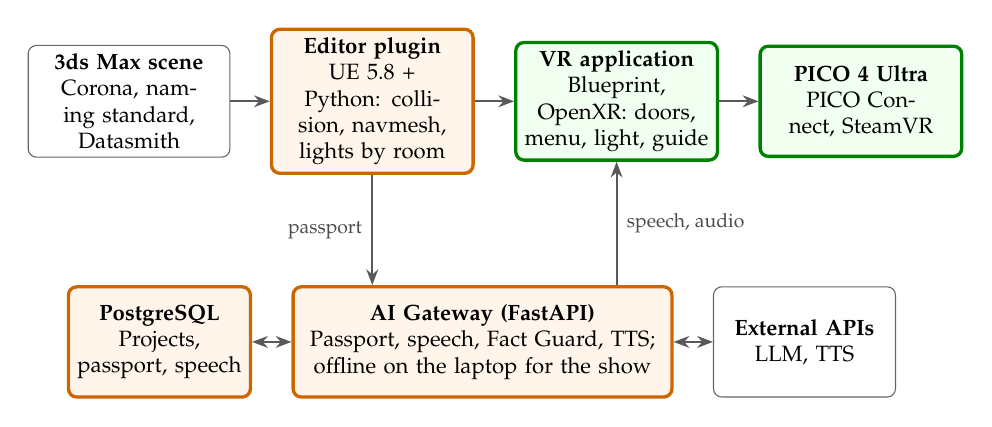
\begin{tikzpicture}[
  node distance=6mm and 5mm,
  box/.style={draw, rounded corners=3pt, align=center, font=\footnotesize, minimum height=14mm, text width=2.35cm, inner sep=3pt},
  done/.style={box, very thick, draw=green!50!black, fill=green!6},
  part/.style={box, very thick, draw=orange!80!black, fill=orange!8},
  ext/.style={box, draw=black!60},
  arr/.style={-{Stealth[length=2mm]}, thick, black!65},
  lbl/.style={font=\scriptsize, text=black!70}
]
\node[ext]  (max)  {\textbf{3ds Max scene}\\Corona, naming standard, Datasmith};
\node[part, right=of max] (plg) {\textbf{Editor plugin}\\UE 5.8 + Python: collision, navmesh, lights by room};
\node[done, right=of plg] (vr)  {\textbf{VR application}\\Blueprint, OpenXR: doors, menu, light, guide};
\node[done, right=of vr]  (hmd) {\textbf{PICO 4 Ultra}\\PICO Connect, SteamVR};
\node[part, below=14mm of plg, xshift=14mm, text width=4.6cm] (gw) {\textbf{AI Gateway (FastAPI)}\\Passport, speech, Fact Guard, TTS; offline on the laptop for the show};
\node[part, left=of gw, text width=2.1cm] (db) {\textbf{PostgreSQL}\\Projects, passport, speech};
\node[ext, right=of gw, text width=2.1cm] (api) {\textbf{External APIs}\\LLM, TTS};
\draw[arr] (max) -- (plg);
\draw[arr] (plg) -- (vr);
\draw[arr] (vr) -- (hmd);
\draw[arr] (plg.south) -- node[lbl, left] {passport} (plg.south |- gw.north);
\draw[arr] (vr.south |- gw.north) -- node[lbl, right] {speech, audio} (vr.south);
\draw[arr, {Stealth[length=2mm]}-{Stealth[length=2mm]}] (db) -- (gw);
\draw[arr, {Stealth[length=2mm]}-{Stealth[length=2mm]}] (gw) -- (api);
\end{tikzpicture}
\caption[System architecture]{System architecture. Green: working prototype; orange: partly built or new; grey: existing tool or service.}
\label{fig:arch}
\end{figure}

Table~\ref{tab:layers} lists the layers, and Table~\ref{tab:components} the components implemented in the VR prototype under their actual names in the Unreal project.

\begin{table}[H]
\centering
\begin{tightblock}
\begin{tabularx}{\textwidth}{P{2.4cm} P{5.0cm} L}
\toprule
\textbf{Layer} & \textbf{Technologies} & \textbf{Responsibility} \\
\midrule
Source & 3ds Max 2024, Corona 11, Datasmith Exporter, MaxScript & Scene, naming check, export \\
Editor plugin & Unreal Engine 5.8.4, Python, Editor Utility menus & Collision, walkable zones, light grouping by room, passport extraction \\
VR application & UE 5.8.4, OpenXR, Blueprint, UMG, Lumen, Sun \& Sky & Locomotion, doors, menu, light, guide \\
AI Gateway & Python, FastAPI, PostgreSQL 16, Docker Compose & Passport storage, speech generation, Fact Guard, TTS, audio files \\
External & LLM API, TTS service & Text and voice \\
\bottomrule
\end{tabularx}
\end{tightblock}
\caption{System layers}
\label{tab:layers}
\end{table}

\begin{table}[H]
\centering
\begin{tightblock}
\footnotesize
\begin{tabularx}{\textwidth}{P{3.6cm} L}
\toprule
\textbf{Component} & \textbf{Role} \\
\midrule
\texttt{BP\_JK3D\_XRPawn} & Player: stick walking, 45\textdegree{} snap turn on the right stick, body capsule against walls, floor safety (return to the last valid point), door push-back, menu laser \\
\texttt{BP\_MovablePart}, \texttt{FindDoor} & Door hinge; the door the hand points at within 150\,cm opens on the trigger, with either hand, from both sides \\
\texttt{BP\_Menu}, \texttt{WBP\_Menu} & VR menu 1.5\,m in front: sun slider 06--22\,h, temperature slider 2700--6500\,K with $\pm$100\,K buttons, room on/off, all on/off \\
\texttt{BP\_JK3D\_Scene} & Room and global light events: \texttt{RoomLightOn/Off}, \texttt{AllLightsOn/Off}, \texttt{SetLightTemp} for the current room \\
\texttt{BP\_JK3D\_LightRoom} & One per room: stores its own temperature and scenario mask, \texttt{ApplyAll} \\
\texttt{BP\_JK3D\_LightSwitch} & Wall switch cycling scenarios 1, 2, 3, all on, all off (postponed for the show) \\
\texttt{BP\_JK3D\_Guide} & Robot guide: follows on the left, waits near objects, stays still while the menu is open, waves once, subtitle queue with a 3\,s minimum \\
\texttt{jk3d\_lighting.py}, \texttt{JK3D\_Collision.py} & Editor scripts: find rooms by \texttt{ROOM\_<ROOM>\_FLOOR}, assign lights to scenarios by name or height, check the collision of all meshes \\
\bottomrule
\end{tabularx}
\end{tightblock}
\caption{Implemented components of the VR prototype}
\label{tab:components}
\end{table}

%----------------------------------------------------------------------------------------
\section{Technology Selection}

\begin{table}[H]
\centering
\begin{tightblock}
\footnotesize
\begin{tabularx}{\textwidth}{P{2.1cm} P{2.6cm} P{2.1cm} L}
\toprule
\textbf{Decision} & \textbf{Chosen} & \textbf{Alternatives} & \textbf{Reason} \\
\midrule
Engine & Unreal Engine 5.8 & Unity, Godot & Datasmith imports 3ds Max/Corona scenes with hierarchy and partial material support; Lumen real-time global illumination; free under USD 1 million revenue \\
Scene transfer & Datasmith & FBX & Keeps lights, cameras and hierarchy; can be automated from Python \\
Headset & PICO 4 Ultra via PICO Connect and SteamVR & Meta Quest 3 & Available to the author; PC rendering keeps Lumen quality \\
VR logic & Blueprint & C++ & Fast iteration, editable through the MCP bridge; C++ only if profiling requires it \\
Backend & FastAPI & Django, Node.js & Async, automatic OpenAPI documentation, same language as the editor scripts \\
Database & PostgreSQL & SQLite, MongoDB & Relational passport data with constraints; JSON fields for flexible values \\
Guide grounding & Approved passport + Fact Guard & Free LLM answers, RAG only & LLMs hallucinate even with retrieval; numbers must be checked after generation \\
Deployment & Docker Compose on a small VPS; local Docker for the demo & Cloud PaaS & Cheap, reproducible, runs offline on the laptop \\
\bottomrule
\end{tabularx}
\end{tightblock}
\caption{Technology choices and their justification}
\label{tab:tech}
\end{table}

%----------------------------------------------------------------------------------------
\section{Data Model and Interfaces}

The AI Gateway stores five entities (Table~\ref{tab:entities}) and exposes a versioned REST API (Table~\ref{tab:api}). All requests except the health check require an API key header; keys and provider tokens live only in server environment variables.

\begin{table}[H]
\centering
\begin{tightblock}
\footnotesize
\begin{tabularx}{\textwidth}{P{2.4cm} P{5.2cm} L}
\toprule
\textbf{Entity} & \textbf{Key fields} & \textbf{Rules} \\
\midrule
\texttt{project} & id, name, brand, address, floor, languages, approved & id unique; languages ISO 639-1 \\
\texttt{passport\_field} & project\_id, key, room, value, unit, source, status, required & (project\_id, key) unique; approval blocked while a required field is empty; any change resets approval \\
\texttt{key\_point} & project\_id, room, language, text, order & written by the designer \\
\texttt{speech} & project\_id, room, language, text, status, fact\_check & only approved speech is voiced and exported \\
\texttt{audio} & speech\_id, voice, file path, MIME type & WAV for direct import into Unreal \\
\bottomrule
\end{tabularx}
\end{tightblock}
\caption{Database entities of the AI Gateway}
\label{tab:entities}
\end{table}

\begin{table}[H]
\centering
\begin{tightblock}
\footnotesize
\begin{tabularx}{\textwidth}{P{4.8cm} L P{3.6cm}}
\toprule
\textbf{Endpoint} & \textbf{Purpose} & \textbf{Main errors} \\
\midrule
\texttt{POST /v1/projects} & Create a project & 409 exists, 422 invalid \\
\texttt{PUT /v1/projects/\{id\}/passport} & Upload passport fields from the plugin & 404, 422 \\
\texttt{PUT /v1/projects/\{id\}/key-points} & Replace the designer's key points & 404, 422 \\
\texttt{POST /v1/projects/\{id\}/approve} & Approve the passport & 409 required field empty \\
\texttt{POST /v1/speech} & Speech per room and language with Fact Guard & 409 not approved, 422 unsupported numbers \\
\texttt{POST /v1/speech/\{id\}/approve} & Approve a speech & 404 \\
\texttt{POST /v1/tts} & Voice an approved speech & 409 not approved, 502 TTS failure \\
\texttt{GET /v1/audio/\{id\}} & Download audio & 404 \\
\texttt{GET /v1/projects/\{id\}/export} & Approved speech and audio for the VR app & 404 \\
\texttt{GET /health} & Health check including the database & -- \\
\bottomrule
\end{tabularx}
\end{tightblock}
\caption{AI Gateway API, version 1}
\label{tab:api}
\end{table}

\paragraph{Fact Guard rule.} Every number in the generated speech must equal a passport value, or the passport value rounded to the number of decimals used in the speech (2.9\,m is supported by 2.89\,m, 3.0\,m is not). Any other number makes the speech fail and return to the designer. For example, \enquote{the living room is 18.4\,\sqm{}} is accepted, while \enquote{the living room is 25\,\sqm{}, renovation takes 30 days} is rejected. A known limitation is that numbers written as words are not detected, so the LLM prompt requires digits.

%----------------------------------------------------------------------------------------
\section{Infrastructure and Facilities}

\begin{table}[H]
\centering
\begin{tightblock}
\begin{tabularx}{\textwidth}{P{3.4cm} L P{2.6cm}}
\toprule
\textbf{Item} & \textbf{Specification} & \textbf{Status} \\
\midrule
Workstation & Author's laptop with an NVIDIA GPU; an audit on 27.10.2026 confirmed it is sufficient & Available \\
Headset & PICO 4 Ultra, PC link through PICO Connect and SteamVR, OpenXR & Available \\
Display for the committee & TV or projector over HDMI & To check before the pre-defense \\
Development bridge & \texttt{unreal-engine-mcp} over the Remote Control API (localhost only) & Working \\
Backend (demo) & Docker on the laptop, works offline & Implemented, 20 tests \\
Backend (production) & VPS 2 vCPU / 4 GB, Ubuntu, Docker Compose, Nginx and Let's Encrypt & Planned \\
Source control & GitHub repository \texttt{kiyalbekkyzy/jk3d-vr} with Git LFS rules for Unreal assets & Created \\
\bottomrule
\end{tabularx}
\end{tightblock}
\caption{Infrastructure and facilities}
\label{tab:infra}
\end{table}

%----------------------------------------------------------------------------------------
\section{MVP and Prototype Status}

The MVP for the diploma has ten functions. Table~\ref{tab:mvp} shows their state on 24 November 2026.

\begin{table}[H]
\centering
\begin{tightblock}
\footnotesize
\begin{tabularx}{\textwidth}{P{0.4cm} P{4.2cm} P{3.0cm} L}
\toprule
\textbf{\#} & \textbf{Function} & \textbf{Status} & \textbf{Evidence} \\
\midrule
1 & Prepare VR: import, collision, navigation, start point & Partly automated & Collision script checked 463 meshes; navigation limited to floor level \\
2 & Walkable zones, automatic and manual & Working; manual editing in the editor & Door openings walkable after excluding door leaves from navigation \\
3 & Opening constructor, 5 techniques & Swing doors only & 6 doors, either hand, both sides, push-back \\
4 & Opening collision check & Not started & -- \\
5 & Light and time & Working (basic) & Sun slider; per-room temperature remembered; 271 lights in 5 rooms; 3 scenarios by naming \\
6 & Project passport & Extracted from the scene; stored and approved on the server & Rooms, lights and doors via the editor; areas to confirm \\
7 & AI guide in Russian and English with voice & Character working; server ready; VR link in progress & Follow, subtitles, wave; 20 backend tests \\
8 & Finish variants & Pre-defense 2 & -- \\
9 & Designer screen and TV mirror & Pre-defense 2 & -- \\
10 & Post-show report & Pre-defense 2 & -- \\
\bottomrule
\end{tabularx}
\end{tightblock}
\caption{MVP functions and their status}
\label{tab:mvp}
\end{table}

Problems solved so far include players getting stuck in door openings (the navigation mesh had holes under closed door leaves), players spawning on the roof (the navigation volume covered the roof), an unreadable VR menu under bright sun (fixed with an exposure-compensated widget material), and room temperature not being saved when the menu was out of view (the widget did not update off-screen).

%----------------------------------------------------------------------------------------
\section{Budget and Resources}

The prototype needs almost no new spending because the laptop and headset are available (Table~\ref{tab:budget}). Prices are as of November 2026 and rounded.

\begin{table}[H]
\centering
\begin{tightblock}
\begin{tabularx}{\textwidth}{P{4.0cm} P{4.4cm} L}
\toprule
\textbf{Item} & \textbf{Cost} & \textbf{Note} \\
\midrule
Laptop with NVIDIA GPU & 0 (available) & Confirmed sufficient \\
PICO 4 Ultra & 0 (available); retail EUR 599 & -- \\
3ds Max & 0 with the Autodesk education licence & Commercial: about USD 2{,}010 per year \\
Unreal Engine 5.8 & 0 under USD 1 million revenue & Epic licence \\
VPS 2 vCPU / 4 GB & about EUR 4--6 per month & Hetzner cost-optimised plan \\
Domain and TLS & about USD 12 per year; TLS free & Approximate \\
LLM API for guide scripts & under USD 1 per project & Estimate; to be measured \\
Text-to-speech & 0 for the prototype & Licence to check before commercial use \\
Cables, HDMI, accessories & about USD 50 & Approximate \\
\midrule
\textbf{Total new spending} & \textbf{about USD 150--200} & To the final defense \\
\bottomrule
\end{tabularx}
\end{tightblock}
\caption{Budget to the final defense}
\label{tab:budget}
\end{table}

\paragraph{Unit economics (hypotheses).} Preparing one presentation costs about 30 minutes of designer time, under USD 1 of API use and a small share of the server. Two revenue models will be tested: a paid VR presentation as an add-on to a design project, and a monthly plugin subscription for studios. Prices are not set yet; they will be asked in 5--10 studio interviews and compared with the current alternatives (panoramas included in the design fee, a Matterport scan at about 5{,}000 KGS, manual tours from USD 10{,}000).

%----------------------------------------------------------------------------------------
\section{Risks}

\begin{table}[H]
\centering
\begin{tightblock}
\begin{tabularx}{\textwidth}{P{5.0cm} L}
\toprule
\textbf{Risk} & \textbf{Mitigation} \\
\midrule
Headset link unstable on demo day & Offline build, recorded video as plan B, cables tested in advance \\
Dynamic light drops FPS below 72 & Lumen Lite, MegaLights, fewer shadowed lights; baked scenarios as fallback \\
Too many features for the time & Strict MVP; finish variants, designer screen and report moved to pre-defense 2 \\
LLM states wrong facts & Approved passport, Fact Guard and designer approval \\
Library furniture is one mesh, fronts cannot open & Openings only for own cabinetry; library items stay static \\
Authorship of AI-assisted work & Git history, work log, AI-use disclosure, the author explains each mechanism \\
\bottomrule
\end{tabularx}
\end{tightblock}
\caption{Risks and mitigation}
\label{tab:risks}
\end{table}
 % Section 3. Methods and Material

\appendix

\chapter{Working Process and Use of AI Tools}
\label{AppendixA}

The project was developed by the author with Claude (Anthropic) as an assistant from 29 September 2026. The work went in short cycles: the author set the goal and constraints, the assistant proposed options, the author chose, the assistant implemented or drafted, and the author tested the result in the headset and reported problems.

\begin{table}[H]
\centering
\begin{tightblock}
\footnotesize
\begin{tabularx}{\textwidth}{P{1.9cm} P{2.3cm} L L}
\toprule
\textbf{Period} & \textbf{Stage} & \textbf{What the author did} & \textbf{What the assistant did} \\
\midrule
29 Sep--13 Oct & Idea and feasibility & Defined the service for the design company; collected its tools and workflow & Desk research, feasibility study draft \\
14 Oct & Research & Chose priorities (quality, budget, timeline) & Compared engines, headsets, AI guide approaches, budget scenarios \\
27--30 Oct & Pilot setup & Installed software, prepared and exported the 3ds Max scene, imported it into Unreal & Step-by-step instructions, troubleshooting \\
30 Oct & Pivot & Changed the idea to an automated plugin for any project & Analysis of analogues, plugin versus standalone, new plan \\
31 Oct--14 Nov & Architecture and MVP & Chose MVP features, naming standard, opening techniques, lighting concept & Architecture, UML diagrams, MVP and weekly plan \\
11--19 Nov & VR prototype & Tested every change in PICO 4 Ultra, chose the menu design and the guide character, reported every bug & Built and connected Blueprint nodes through the MCP bridge, diagnosed causes, kept the work log \\
24 Nov & Backend and report & Chose the project category, created the GitHub repository, reviewed results & AI Gateway code and tests, report draft, progress report \\
\bottomrule
\end{tabularx}
\end{tightblock}
\caption{Division of work between the author and the AI assistant}
\label{tab:ai-work}
\end{table}

\paragraph{Rules the author followed.} Every change was tested in the headset before it was accepted; every bug was logged as problem, cause, fix and result; backups were made before each editing session; all design decisions were made by the author. The text of this report will be rewritten by the author in her own words, and the chat history is kept as required by the university guideline.

\section*{Evidence}

% Insert screenshots of the chat history here, e.g.:
% \begin{figure}[H]\centering\includegraphics[width=\textwidth]{Figures/chat1.png}\caption{Setting the task and first research, 14 Oct 2026}\end{figure}
\begin{enumerate}
\item Screenshot: setting the task and first research (14 October 2026).
\item Screenshot: the pivot to an automated plugin (30 October 2026).
\item Screenshot: choosing the MVP features and the lighting concept.
\item Screenshot: choosing the VR menu design (variant C).
\item Screenshot: choosing the guide character.
\item Screenshot: a bug report from a headset test and its fix (19 November 2026).
\item Screenshot: backend tests passing (24 November 2026).
\end{enumerate}
 % Working process and use of AI tools
\chapter{Plan to Pre-Defense 2 and the Final Defense}
\label{AppendixB}

By April 2027 (80--90\% readiness) the core functions, the backend with tests and the first user evaluation must be complete.

\begin{table}[H]
\centering
\begin{tightblock}
\begin{tabularx}{\textwidth}{P{2.8cm} L P{3.6cm}}
\toprule
\textbf{Period} & \textbf{Work} & \textbf{Result} \\
\midrule
24--30 Nov 2026 & AI Gateway v1; guide voice in VR; GitHub repository; slides; plan B video & Pre-defense 1 demo \\
Dec 2026 & Opening techniques 2--5; opening collision check; second 3ds Max project & First measurement for RQ1 \\
Jan 2027 & Designer screen and TV mirror; finish variants; \enquote{Prepare VR} in one menu & Full show flow \\
Feb 2027 & Post-show report; automated tests; VPS deployment with CI/CD & Reproducible release \\
Mar 2027 & User study (5+ participants), studio interviews, company letters & Data for RQ2 and RQ3 \\
Apr 2027 & Sections 3--4 of the report & Pre-defense 2 \\
May 2027 & Section 5; final report uploaded by 10--15 May & Final defense, 1--5 June 2027 \\
\bottomrule
\end{tabularx}
\end{tightblock}
\caption{Work plan to the final defense}
\label{tab:plan}
\end{table}
 % Plan to pre-defense 2

\bibliography{references}

\end{document}
